\chapter{الكيمياء البيئية وعلم السموم}\label{ch:b3:environmental-toxicology}

في أواخر كل صيف، تصوّر الأقمار الاصطناعية دوامات خضراء تنتشر على البحيرات
الكبيرة: إنها أزهار طحالب يغذيها الفوسفات والنترات اللذان يجرفهما الماء من الحقول
ويخرجان من المدن. وحين تموت الطحالب وتغوص، يستهلك تحللها أكسجين
المياه العميقة، فتموت الأسماك. والكيمياء تفسّر كل حلقة من هذه السلسلة، ومن
سلاسل أخرى كثيرة: لماذا تُدفئ بعض الغازات الكوكب ولا تدفئه أخرى، ولماذا يكون المطر
حمضيًا حتى في الهواء النظيف، وأين ينتهي المبيد بعد رشه، وكم
يلزم من مادة ما لتُحدث ضررًا. ويطبّق هذا الفصل التوازنات
والحركية والمطيافية على الغلاف الجوي والمياه الطبيعية والتربة، ويتتبع
الملوثات بينها، وينتهي بالأرقام التي تُبنى عليها تقييمات
المخاطر.

\begin{recall}
عالج مجلد السنة الأولى توازنات الحمض--القاعدة والترسيب والتعقيد،
ومخططات الجهد--pH، ومعاملات التوزيع، وأعمار النصف، والخطر،
والمخاطرة ونظام GHS؛ وعالج المجلد المدرسي غازات الدفيئة؛ ومجلد السنة الثانية
قانون هنري، والقوة الأيونية، والإحصاء، ومطيافية الكتلة والمطيافية
الذرية. وعالجت \cref{ch:b3:photochemistry} الكيمياء الضوئية للغلاف الجوي،
و\cref{ch:b3:group-theory-applied} و\cref{ch:b3:rovibrational-spectroscopy}
النشاط في تحت الأحمر، و\cref{ch:b3:surfaces-catalysis} \omterm{def:b3:surfaces-catalysis:adsorption}{الامتزاز}.
\end{recall}

\begin{omfigure}
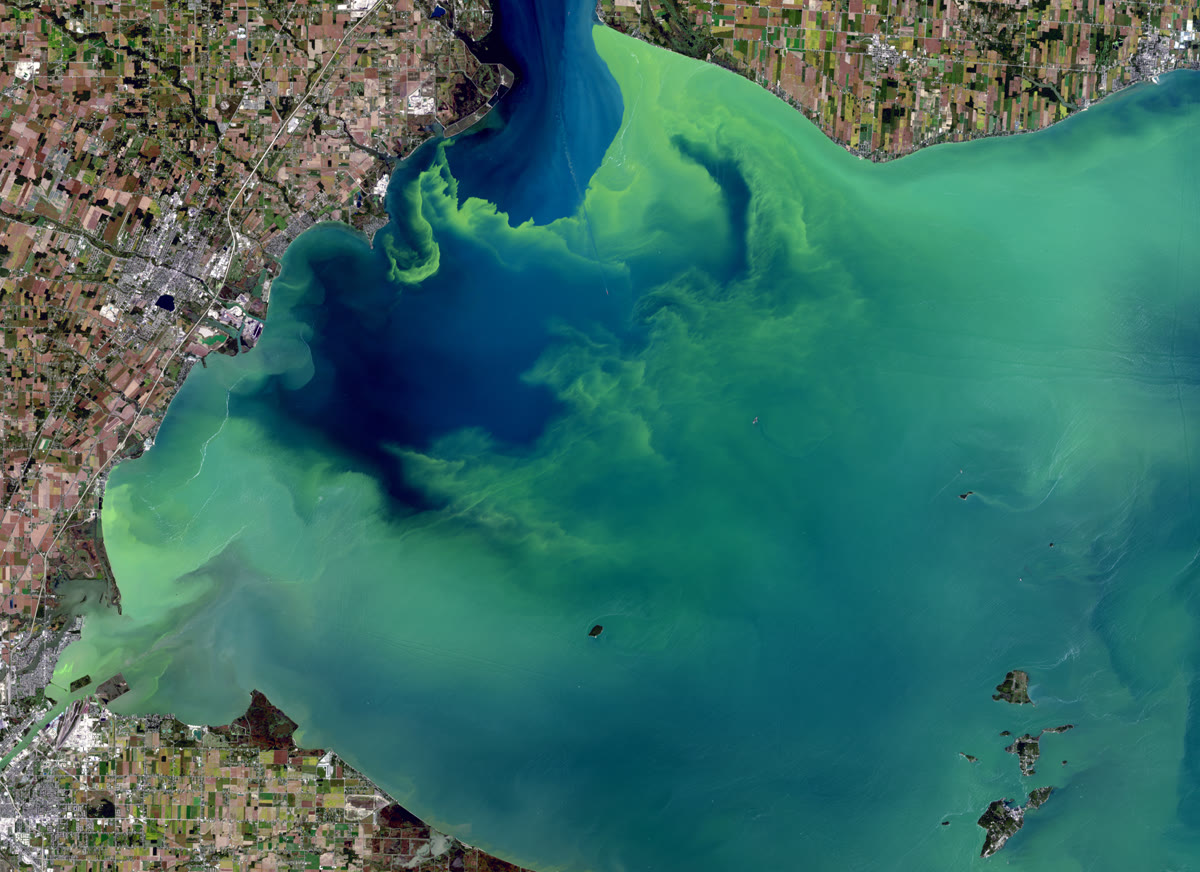
\includegraphics[width=0.62\linewidth]{images/book4/algal-bloom.jpg}

{\small زهرة طحالب على بحيرة كبيرة، كما رآها قمر اصطناعي لرصد الأرض في
أواخر أيلول/سبتمبر: الدوامات الخضراء تجمعات كثيفة من طحالب مجهرية
تغذيها المغذيات الآتية من الأراضي الزراعية المحيطة. الصورة: USGS وNASA، ملك عام.}
\end{omfigure}

\section{الغلاف الجوي}

\begin{definition}[غازات الدفيئة]\label{def:b3:environmental-toxicology:greenhouse}
\emph{غاز الدفيئة}\index{غاز دفيئة} غاز يمتص الأشعة تحت الحمراء ويصدرها
عند أطوال موجات الإشعاع الصادر عن سطح الأرض، فيُدفئ
بذلك الغلاف الجوي السفلي. و\emph{قدرة الاحترار
العالمي}\index{قدرة الاحترار العالمي} (GWP) لغاز ما على أفق زمني،
هو عادة 100 سنة، هي الطاقة التي يحتجزها بعد انبعاث كيلوغرام واحد منه،
نسبةً إلى كيلوغرام واحد من ثنائي أكسيد الكربون.
\end{definition}

لا يمتص الجزيء الأشعة تحت الحمراء إلا عبر اهتزازات تغيّر
عزمه ثنائي القطب (\cref{ch:b3:group-theory-applied}). وثنائي النيتروجين وثنائي الأكسجين،
وهما جزيئان ثنائيا الذرة متجانسا النواة، لا يملكان مثل هذا الاهتزاز فهما شفافان؛ والأرغون لا يملك
أي اهتزاز أصلًا. أما ثنائي أكسيد الكربون، الخطي وغير القطبي، فله نمط انحناء
\omterm{def:b3:group-theory-applied:activity}{نشط في تحت الأحمر} قرب \qty{15}{\micro\metre}، في وسط إصدار الأرض؛ والماء والميثان
وأكسيد النيتروز تمتص عند أطوال موجات كثيرة.

% ledger: atm:CO2.2025, atm:CH4.2025, atm:N2O.2025, gwp:CH4.fossil, gwp:CH4.nonfossil, gwp:N2O, life:CH4, life:N2O
في سنة 2025 كانت الكسور المولية المتوسطة العالمية \qty{425.6}{ppm} لثنائي أكسيد الكربون، و\qty{1936}{ppb}
للميثان و\qty{338.9}{ppb} لأكسيد النيتروز. والميثان، الذي تزيله جذور الهيدروكسيل
بعمر نحو 12 سنة، له قدرة احترار عالمي على مئة سنة من 27 إلى 30؛ وأكسيد النيتروز، الذي لا يُتلف إلا في
الستراتوسفير بعمر نحو 109 سنوات، له 273. وليس لثنائي أكسيد الكربون
عمر واحد: فجزء من الانبعاث يبقى في الهواء قرونًا.

\begin{definition}[ملوثات الهواء]\label{def:b3:environmental-toxicology:pollutants}
\emph{الجسيمات العالقة}\index{جسيمات عالقة} هي الجسيمات الصلبة والسائلة
المعلقة في الهواء، وتُصنَّف بحسب قطرها الديناميكي الهوائي (فالجسيمات الدقيقة
التي يقل قطرها عن \qty{2.5}{\micro\metre} تبلغ أعماق الرئتين). و\emph{المطر
الحمضي}\index{مطر حمضي} مطر صار أكثر حمضية من المطر النظيف بحمضي الكبريتيك
والنتريك المتكوّنين من ثنائي أكسيد الكبريت وأكاسيد النيتروجين.
\end{definition}

\begin{proposition}[pH المطر النظيف]\label{prop:b3:environmental-toxicology:rain-ph}
المطر المتوازن مع ثنائي أكسيد الكربون في هواء اليوم، ومع لا شيء
سواه، قيمة pH له نحو 5.6.
\end{proposition}

\begin{proof}
% ledger: henry:CO2, pka4:H2CO3.1, pkw4:25C, const:atm
يعطي قانون هنري $[\ce{CO2(aq)}] = K_Hp(\ce{CO2}) = \qty{3.4e-7}{mol.L^{-1}.Pa^{-1}} \times (425.6 \times 10^{-6} \times \qty{101325}{Pa}) = \qty{1.47e-5}{mol/L}$. 
وموازنة الشحنات هي $[\ce{H+}] = [\ce{HCO3-}] + 2[\ce{CO3^2-}] + [\ce{OH-}] \approx K_{a1}[\ce{CO2(aq)}]/[\ce{H+}] + K_w/[\ce{H+}]$، ومنها
$[\ce{H+}]^2 = K_{a1}[\ce{CO2(aq)}] + K_w = 10^{-6.35} \times \num{1.47e-5} + 10^{-14} = \num{6.6e-12}$: $[\ce{H+}] = \qty{2.6e-6}{mol/L}$، وpH يساوي 5.6.
\end{proof}

يتأكسد ثنائي أكسيد الكبريت الآتي من حرق الوقود المحتوي على الكبريت وأكاسيد النيتروجين الآتية من
الاحتراق الساخن في الهواء، بجذور الهيدروكسيل وفي قطيرات
السحب، إلى حمضي الكبريتيك والنتريك، اللذين يخفضان pH المطر إلى 4 وما دونها.
وقد حلّت إزالةُ الكبريت من الوقود وأكاسيد النيتروجين من غازات العادم (المحولات
الحفزية، وحقن الأمونيا في محطات توليد الكهرباء) المشكلةَ إلى حد كبير
حيث طُبّقت. ويبقى الأوزون قرب سطح الأرض، المتكوّن حين يؤثر ضوء الشمس في
أكاسيد النيتروجين والمركبات العضوية المتطايرة (\cref{ch:b3:photochemistry})، 
والجسيمات الدقيقة، ملوثات الهواء الرئيسة على الصحة.

\section{المياه الطبيعية}

\begin{omfigure}
\begin{tikzpicture}
\begin{axis}[name=a, width=0.48\linewidth, height=5.4cm, xmin=4, xmax=13, ymin=0, ymax=1.02,
  axis lines=left, xlabel={\babelsublr{pH}}, ylabel={\foreignlanguage{arabic}{جزء الكربون المذاب}},
  tick label style={font=\scriptsize}, label style={font=\small}]
\addplot[color=omDef, thick] table[x=pH, y=a0] {figdata/out/bachelor-3-carbonate-system.dat};
\addplot[color=omMeth, thick] table[x=pH, y=a1] {figdata/out/bachelor-3-carbonate-system.dat};
\addplot[color=omThm, thick] table[x=pH, y=a2] {figdata/out/bachelor-3-carbonate-system.dat};
\node[font=\scriptsize, omDef] at (axis cs:4.9,0.85) {$\ce{CO2(aq)}$};
\node[font=\scriptsize, omMeth] at (axis cs:8.3,0.88) {$\ce{HCO3-}$};
\node[font=\scriptsize, omThm] at (axis cs:12.1,0.85) {$\ce{CO3^2-}$};
\draw[black!30, dashed] (axis cs:6.35,0) -- (axis cs:6.35,0.5) (axis cs:10.33,0) -- (axis cs:10.33,0.5);
\end{axis}
\begin{axis}[at={(a.east)}, anchor=west, xshift=1.4cm, width=0.48\linewidth, height=5.4cm,
  xmin=0, xmax=2000, ymin=5.2, ymax=6.2, axis lines=left,
  xlabel={\foreignlanguage{arabic}{$\ce{CO2}$ في الهواء، بأجزاء في المليون}}, ylabel={\foreignlanguage{arabic}{قيمة pH للمطر}},
  tick label style={font=\scriptsize}, label style={font=\small},
  scaled x ticks=false, xticklabel style={/pgf/number format/1000 sep={}}]
\addplot[color=omDef, thick] table[x=ppm, y=pH] {figdata/out/bachelor-3-carbonate-system-b.dat};
\draw[black!35, dashed] (axis cs:425.6,5.2) -- (axis cs:425.6,5.59);
\node[font=\scriptsize, anchor=west] at (axis cs:470,5.63) {\foreignlanguage{arabic}{اليوم: 5.6}};
\end{axis}
\end{tikzpicture}

{\small يسارًا: توزع الكربون غير العضوي المذاب بين صوره الثلاث
بدلالة pH عند \qty{25}{\celsius}، مع تقاطعات عند $\mathrm pK_{a1} = 6.35$ و$\mathrm pK_{a2} = 10.33$. يمينًا: قيمة pH للمطر
المتوازن مع ثنائي أكسيد الكربون وحده، بدلالة كسره المولي في الهواء.}
\end{omfigure}

\begin{proposition}[أجزاء الكربونات]\label{prop:b3:environmental-toxicology:carbonate-fractions}
إذا كان $C_T$ الكربون غير العضوي المذاب الكلي، فإن
$[\ce{CO2(aq)}] = C_Th^2/D$، و$[\ce{HCO3-}] = C_TK_{a1}h/D$، و$[\ce{CO3^2-}] = C_TK_{a1}K_{a2}/D$، حيث $h = [\ce{H+}]$ و$D = h^2 + K_{a1}h + K_{a1}K_{a2}$.
\end{proposition}

\begin{proof}
من ثابتي الحموضة،
\[
  [\ce{HCO3-}] = \frac{K_{a1}[\ce{CO2(aq)}]}{h}, \qquad [\ce{CO3^2-}] = \frac{K_{a2}[\ce{HCO3-}]}{h} = \frac{K_{a1}K_{a2}[\ce{CO2(aq)}]}{h^2}.
\]
مجموعها $C_T = [\ce{CO2(aq)}]\,D/h^2$؛ وقسمة كل صورة على $C_T$ تعطي الأجزاء.
\end{proof}

\begin{definition}[القلوية]\label{def:b3:environmental-toxicology:alkalinity}
\emph{قلوية}\index{قلوية} الماء هي قدرته على معادلة
حمض قوي، وتُقاس بالمعايرة حتى نقطة نهاية حمض الكربونيك (عند pH نحو
4.5) ويُعبَّر عنها بمولات $\ce{H+}$ لكل لتر.
\end{definition}

\begin{proposition}[قلوية الكربونات]\label{prop:b3:environmental-toxicology:alkalinity}
في ماء قواعده هي أنواع الكربونات والهيدروكسيد،
$\mathrm{Alk} = [\ce{HCO3-}] + 2[\ce{CO3^2-}] + [\ce{OH-}] - [\ce{H+}]$؛ وهي تساوي زيادة شحنات كاتيونات القواعد القوية
على شحنات أنيونات الأحماض القوية، ولا تتغير حين يتبادل الماء
ثنائي أكسيد الكربون مع الهواء.
\end{proposition}

\begin{proof}
تحوّل المعايرة حتى نقطة نهاية حمض الكربونيك كل $\ce{HCO3-}$ إلى $\ce{CO2}$ (بأيون $\ce{H+}$ واحد لكل منها)،
وكل $\ce{CO3^2-}$ إلى $\ce{CO2}$ (باثنين)، وكل $\ce{OH-}$ إلى ماء (بواحد)، بينما تُحسب أيونات $\ce{H+}$ الحرة الموجودة أصلًا
بالسالب: وهذا هو المجموع المذكور. وموازنة شحنات الماء، مع
$\ce{Na+}$ و$\ce{Ca^2+}$\dots{} و$\ce{Cl-}$ و$\ce{SO4^2-}$\dots، يُعاد ترتيبها إلى المجموع نفسه، مساويًا $\sum z_i c_i$ (للكاتيونات) $-$ $\sum z_jc_j$ (للأنيونات)
للإلكتروليتات القوية. وإضافة $\ce{CO2}$ أو إزالته لا تغيّر أيًا من هذه الأيونات.
\end{proof}

\begin{definition}[تحمض المحيطات]\label{def:b3:environmental-toxicology:acidification}
\emph{تحمض المحيطات}\index{تحمض المحيطات} هو انخفاض
pH ماء البحر حين يمتص ثنائي أكسيد الكربون من الهواء. و\emph{حالة
التشبع}\index{حالة التشبع} لمعدن كربوناتي هي
$\Omega = [\ce{Ca^2+}][\ce{CO3^2-}]/K_{sp}$: فوق 1 يمكن أن يتكوّن المعدن، وتحت 1 يميل إلى الذوبان.
\end{definition}

يحوّل ثنائي أكسيد الكربون المذاب أيونات الكربونات إلى هيدروجين كربونات، $\ce{CO2 + CO3^2- + H2O -> 2HCO3-}$،
فيخفض pH و$\Omega$: فيصير بناء الأصداف وهياكل المرجان أصعب. (في
ماء البحر تكون الثوابت ظاهرية، مقيسة في الوسط الملحي، 
وتختلف عن قيم الماء العذب المستعملة في هذا الفصل.)

\begin{definition}[عسر الماء]\label{def:b3:environmental-toxicology:hardness}
\emph{عسر}\index{عسر الماء} الماء هو التركيز الكلي
لأيونات الكالسيوم والمغنيسيوم فيه، ويُعبَّر عنه غالبًا بكتلة كربونات الكالسيوم
التي تحتوي العدد نفسه من المولات، بالمليغرام لكل لتر.
\end{definition}

\begin{definition}[الطلب على الأكسجين]\label{def:b3:environmental-toxicology:oxygen-demand}
\emph{الطلب البيوكيميائي على الأكسجين}\index{طلب بيوكيميائي على الأكسجين} (BOD) لماء ما
هو كتلة ثنائي الأكسجين التي تستهلكها في اللتر الواحد الكائنات الدقيقة وهي تؤكسد
مادته العضوية في الظلام، خلال زمن محدد (خمسة أيام عند \qty{20}{\celsius} من أجل $\mathrm{BOD_5}$). 
و\emph{الطلب الكيميائي على الأكسجين}\index{طلب كيميائي على الأكسجين} (COD) هو كتلة
ثنائي الأكسجين المكافئة للديكرومات المستهلَكة في أكسدة مادته العضوية
كيميائيًا.
\end{definition}

\begin{proposition}[منحنى الطلب البيوكيميائي على الأكسجين]\label{prop:b3:environmental-toxicology:bod}
إذا استُهلكت المادة العضوية القابلة للتحلل الحيوي وفق حركية من الرتبة الأولى بثابت
سرعة $k$، فإن الأكسجين المستعمل بعد زمن $t$ هو $\mathrm{BOD}_t = L_0(1 - \eu^{-kt})$، حيث $L_0$ هو الطلب البيوكيميائي النهائي.
\end{proposition}

\begin{proof}
الطلب المتبقي $L$ يحقق $\dd L/\dd t = -kL$، ومنه $L = L_0\eu^{-kt}$؛ والأكسجين المستعمل هو ما ذهب منه،
أي $L_0 - L$.
\end{proof}

\begin{omfigure}
\begin{tikzpicture}
\begin{axis}[name=a, width=0.48\linewidth, height=5.2cm, xmin=0, xmax=30, ymin=0, ymax=270,
  axis lines=left, xlabel={\foreignlanguage{arabic}{الزمن بالأيام}}, ylabel={\babelsublr{BOD / \unit{mg.L^{-1}}}},
  tick label style={font=\scriptsize}, label style={font=\small}]
\addplot[color=omDef, thick] table[x=t, y=bod] {figdata/out/bachelor-3-bod.dat};
\draw[black!35, dashed] (axis cs:0,250) -- (axis cs:30,250);
\draw[black!35, dashed] (axis cs:5,0) -- (axis cs:5,170.8);
\node[font=\scriptsize, anchor=west] at (axis cs:5.6,140) {$\mathrm{BOD_5}$};
\node[font=\scriptsize, anchor=north east] at (axis cs:30,246) {$L_0$};
\end{axis}
\begin{axis}[at={(a.east)}, anchor=west, xshift=1.4cm, width=0.48\linewidth, height=5.2cm,
  xmin=0, xmax=15, ymin=0, ymax=10, axis lines=left,
  xlabel={\foreignlanguage{arabic}{زمن الجريان نحو المصب بالأيام}}, ylabel={\foreignlanguage{arabic}{$\ce{O2}$ المذاب \babelsublr{(\unit{mg.L^{-1}})}}},
  tick label style={font=\scriptsize}, label style={font=\small}]
\addplot[color=omThm, thick] table[x=t, y=O2] {figdata/out/bachelor-3-bod-b.dat};
\draw[black!35, dashed] (axis cs:0,9.1) -- (axis cs:15,9.1);
\node[font=\scriptsize, anchor=south east] at (axis cs:15,9.1) {\foreignlanguage{arabic}{الإشباع}};
\node[font=\scriptsize, anchor=north] at (axis cs:2.4,6.3) {\foreignlanguage{arabic}{النقطة الحرجة}};
\end{axis}
\end{tikzpicture}

{\small يسارًا: \omterm{def:b3:environmental-toxicology:oxygen-demand}{الطلب البيوكيميائي على الأكسجين} لمياه صرف نموذجية، $L_0 = \qty{250}{mg/L}$ و$k = \qty{0.23}{d^{-1}}$: يُستعمل نحو ثلثي
الطلب في خمسة أيام. يمينًا: هبوط الأكسجين في نهر أسفل مصبّ صرف
(نموذج ستريتر--فيلبس): يستهلك تحلل الحمل العضوي الأكسجين أسرع مما
يعيده الهواء في البداية، حتى يبلغ العجز ذروته بعد نحو 2.4 يوم.}
\end{omfigure}

\begin{method}[تعيين الطلب الكيميائي على الأكسجين]\label{met:b3:environmental-toxicology:cod}
\begin{enumerate}
  \item سخّن مع التقطير الارتدادي حجمًا مقيسًا من العينة مع فائض معلوم من ثنائي كرومات
        البوتاسيوم في حمض الكبريتيك، مع كبريتات الفضة حفازًا
        وكبريتات الزئبق(II) لربط الكلوريد.
  \item عاير الديكرومات المتبقية بالحديد(II) باستعمال الفيروين، وأجرِ
        تجربة شاهدة بالماء النقي.
  \item الديكرومات المستهلكة، محوَّلةً إلى الكتلة المكافئة من $\ce{O2}$ (فالأيون
        $\ce{Cr2O7^2-}$ الواحد يأخذ ستة إلكترونات، كما يأخذها 1.5 من $\ce{O2}$)، مقسومةً على حجم العينة، هي
        \omterm{def:b3:environmental-toxicology:oxygen-demand}{الطلب الكيميائي على الأكسجين} بالمليغرام لكل لتر.
\end{enumerate}
\end{method}

\begin{definition}[الإثراء الغذائي]\label{def:b3:environmental-toxicology:eutrophication}
\emph{الإثراء الغذائي}\index{إثراء غذائي} هو إغناء مسطح مائي
بالمغذيات، ولا سيما الفوسفور والنيتروجين، بما يؤدي إلى نمو مفرط
للطحالب والنباتات، ثم إلى استنفاد الأكسجين حين تتحلل.
\end{definition}

\begin{omfigure}
\begin{tikzpicture}[font=\scriptsize, >=Stealth,
  box/.style={draw, rounded corners, align=center, fill=omMeth!10, inner sep=3pt, minimum height=8mm}]
  \node[box] (f) at (-3.4,1.2) {\foreignlanguage{arabic}{الحقول: أسمدة،}\\ \foreignlanguage{arabic}{سماد حيواني}};
  \node[box] (t) at (-3.4,-0.4) {\foreignlanguage{arabic}{المدن: مياه صرف،}\\ \foreignlanguage{arabic}{منظفات}};
  \node[box] (a) at (0,2.1) {\foreignlanguage{arabic}{الغلاف الجوي:}\\ \foreignlanguage{arabic}{ترسّب النيتروجين}};
  \node[box, fill=omDef!12, minimum width=3.2cm, minimum height=1.7cm] (l) at (0.6,0.4) {\foreignlanguage{arabic}{ماء البحيرة:}\\ \foreignlanguage{arabic}{تنمو الطحالب}};
  \node[box, fill=black!8] (s) at (0.6,-1.6) {\foreignlanguage{arabic}{الرواسب: تخزّن الفوسفور،}\\ \foreignlanguage{arabic}{وتطلقه عند انعدام الأكسجين}};
  \node[box] (o) at (4.0,0.4) {\foreignlanguage{arabic}{المخرج}};
  \draw[->, thick] (f) -- node[above, sloped, pos=0.45] {\foreignlanguage{arabic}{الجريان}} (l);
  \draw[->, thick] (t) -- node[below, sloped] {N, P} (l);
  \draw[->, thick] (a) -- (l);
  \draw[->, thick] (l) -- node[left] {\foreignlanguage{arabic}{طحالب ميتة}} (s);
  \draw[->, thick, dashed] (s.east) to[bend right=30] node[right] {P} (l.south east);
  \draw[->, thick] (l) -- (o);
\end{tikzpicture}

{\small تدفقات المغذيات إلى البحيرة وداخلها. فالفوسفور، وهو غالبًا المغذي
المحدِّد في الماء العذب، يتراكم في الرواسب ويعود إلى الماء
حين يفقد القاع أكسجينه، وهذا قد يُبقي الأزهار سنوات بعد
قطع المدخلات.}
\end{omfigure}

تمتص الطحالب الكربون والنيتروجين والفوسفور بنسب ثابتة تقريبًا؛
وأيّ مغذٍّ يقل عن تلك الحاجات يحدّ من نموها. وفي
معظم البحيرات يكون هذا المغذي هو الفوسفور، ولذلك أُزيلت الفوسفات من
المنظفات ومن مياه الصرف المعالجة؛ وفي كثير من البحار الساحلية يكون النيتروجين.

\begin{definition}[الانتواع]\label{def:b3:environmental-toxicology:speciation}
\emph{الانتواع الكيميائي}\index{انتواع كيميائي} لعنصر في
عينة هو توزع كميته على صوره الكيميائية: حالات
الأكسدة، والمعقدات، والمركبات الفلزية العضوية، والأنواع الحرة والمرتبطة.
\end{definition}

تتوقف السمية على الانتواع. فالزئبق غير العضوي المنطلق في الماء
تُمثيله البكتيريا في الرواسب إلى ميثيل الزئبق، الذي يعبر الأغشية،
ويرتبط بكبريت البروتينات ويتركز صعودًا في السلاسل الغذائية؛ والزرنيخ أشد
سمية بكثير في صورة الزرنيخيت، أي الزرنيخ(III)، منه في صورة الزرنيخات، أي الزرنيخ(V)، وأقل سمية بكثير في الصور
العضوية الموجودة في المأكولات البحرية. فالتركيز الكلي وحده لا يقول إلا القليل.

\begin{method}[انتواع فلز في ماء]\label{met:b3:environmental-toxicology:speciation}
\begin{enumerate}
  \item عدّد الربائط الموجودة (الهيدروكسيد، والكربونات، والكلوريد، والكبريتات، والمادة
        العضوية) مع تراكيزها وقيمة pH.
  \item اكتب ثوابت التعقيد وموازنة كتلة الفلز، كما في
        مجلد السنة الأولى.
  \item احسب أيون الفلز الحر، ثم كل معقد؛ وارسم الأجزاء بدلالة
        pH أو بدلالة تركيز ربيطة.
  \item قارن الصورة السامة أو المتاحة حيويًا (وهي غالبًا الأيون الحر) بالمجموع.
\end{enumerate}
\end{method}

\section{التربة والرواسب}

\begin{definition}[الامتزاز في التربة]\label{def:b3:environmental-toxicology:soil}
\emph{سعة التبادل الكاتيوني}\index{سعة التبادل الكاتيوني} للتربة هي
كمية الكاتيونات القابلة للتبادل التي تستطيع الاحتفاظ بها لكل وحدة كتلة، على الطين والمادة
العضوية. و\emph{معامل التوزيع بين التربة والماء}\index{معامل التوزيع بين التربة والماء}
$K_d$ هو نسبة تركيز \omterm{def:b3:surfaces-catalysis:adsorption}{مادة
ممتزة} على التربة (لكل كيلوغرام) إلى تركيزها في ماء المسام (لكل
لتر)؛ و\emph{معامل التوزيع على الكربون العضوي}\index{معامل التوزيع على الكربون العضوي}
هو $K_{oc} = K_d/f_{oc}$، حيث $f_{oc}$ الكسر الكتلي للكربون العضوي.
\end{definition}

تمتز المركبات العضوية المتعادلة أساسًا على المادة العضوية للتربة، بحيث يتغير $K_{oc}$
من تربة إلى أخرى أقل بكثير مما يتغير $K_d$. فالمركب ذو القيمة الصغيرة للثابت $K_d$ يتحرك مع الماء
ويمكن أن يبلغ المياه الجوفية (الارتشاح)؛ أما ذو القيمة الكبيرة للثابت $K_d$ فيبقى قرب السطح،
مرتبطًا بجسيمات قد يحملها الانجراف إلى الأنهار والبحيرات.

\section{مصير الملوثات}

\begin{definition}[معامل التوزيع بين الأوكتانول والماء]\label{def:b3:environmental-toxicology:kow}
\emph{معامل التوزيع بين الأوكتانول والماء}\index{معامل التوزيع بين الأوكتانول والماء}
$K_{ow}$ لمادة ما هو نسبة تركيزيها عند التوازن في
الأوكتان-1-ول وفي الماء؛ وهو يقيس ألفتها للأنسجة الدهنية والمادة
العضوية.
\end{definition}

% ledger: logkow:DDT, logkow:benzene, logkow:atrazine, logkow:PCB153
للبنزين $\log K_{ow} = 2.13$، ولمبيد الأعشاب الأترازين 2.61، ولمركب PCB سداسي الكلور 6.67،
ولمبيد الحشرات DDT 6.91: فالأخيران يذوبان في الدهون أفضل بعشرات ملايين المرات مما يذوبان في
الماء.

\begin{definition}[التراكم الحيوي]\label{def:b3:environmental-toxicology:bio}
\emph{عامل التركيز الحيوي}\index{عامل التركيز الحيوي} (BCF) هو
نسبة التركيز في كائن حي إلى التركيز في الماء المحيط به عند
الحالة المستقرة، حين يكون الامتصاص من الماء وحده. و\emph{التراكم الحيوي}\index{تراكم حيوي}
هو تراكم المادة في الكائن من كل المسالك، بما فيها الغذاء؛
و\emph{التضخم الحيوي}\index{تضخم حيوي} هو ازدياد
التركيز من الفريسة إلى المفترس صعودًا في السلسلة الغذائية.
\end{definition}

\begin{proposition}[عامل التركيز الحيوي و$K_{ow}$]\label{prop:b3:environmental-toxicology:bcf-kow}
بالنسبة إلى المواد العضوية المتعادلة التي لا تُستقلب، يكون $\log\mathrm{BCF}$ في الأسماك
دالة خطية تقريبًا في $\log K_{ow}$، بميل قريب من 1، حتى يبلغ $\log K_{ow}$ نحو 6؛
وفوق ذلك يتباطأ الامتصاص وتستوي العلاقة (انحدارات تجريبية).
\admitted
\end{proposition}

\begin{definition}[الملوثات العضوية الثابتة]\label{def:b3:environmental-toxicology:pop}
\emph{الملوث العضوي الثابت}\index{ملوث عضوي ثابت}
مادة عضوية تقاوم التحلل، وتتراكم حيويًا، وهي سامة
وتُنقل بعيدًا عن مصادرها، مثل DDT ومركبات PCB والديوكسينات.
\end{definition}

\begin{proposition}[التوزع عند التوازن بين الأحياز]\label{prop:b3:environmental-toxicology:level-one}
كتلة $M$ من مادة موزعة عند التوازن (نموذج «المستوى الأول») بين الماء
(الحجم $V_w$)، والهواء ($V_a$)، وجوامد الرواسب ($m_s$) والأسماك ($m_f$) يكون تركيزها في الماء
$C_w = M/(V_w + K_{aw}V_a + K_{sw}m_s + K_{fw}m_f)$، حيث $K$ هي معاملات التوزيع نسبةً إلى
الماء؛ والكتلة في كل حيز هي حدّه مضروبًا في $C_w$.
\end{proposition}

\begin{proof}
عند التوازن $C_a = K_{aw}C_w$، و$C_s = K_{sw}C_w$ (لكل كيلوغرام)، و$C_f = K_{fw}C_w$. وموازنة الكتلة هي
$M = C_wV_w + C_aV_a + C_sm_s + C_fm_f = C_w(V_w + K_{aw}V_a + K_{sw}m_s + K_{fw}m_f)$؛ والقسمة تعطي $C_w$.
\end{proof}

\begin{omfigure}
\begin{tikzpicture}[font=\scriptsize, >=Stealth,
  comp/.style={draw, rounded corners, align=center, minimum width=2.6cm, minimum height=1.0cm}]
  \node[comp, fill=omDef!8] (air) at (0,2.2) {\foreignlanguage{arabic}{الهواء}\\ $C_a = K_{aw}C_w$};
  \node[comp, fill=omDef!25] (w) at (0,0.6) {\foreignlanguage{arabic}{الماء}\\ $C_w$};
  \node[comp, fill=black!10] (sed) at (0,-1.0) {\foreignlanguage{arabic}{الرواسب}\\ $C_s = K_{sw}C_w$};
  \node[comp, fill=omMeth!15] (fish) at (3.6,0.6) {\foreignlanguage{arabic}{الأسماك}\\ $C_f = K_{fw}C_w$};
  \node[comp, fill=omProp!15] (soil) at (-3.6,0.6) {\foreignlanguage{arabic}{التربة}\\ $C_{soil} = K_dC_w$};
  \draw[<->, thick] (air) -- (w); \draw[<->, thick] (w) -- (sed);
  \draw[<->, thick] (w) -- (fish); \draw[<->, thick] (w) -- (soil);
\end{tikzpicture}

{\small أحياز نموذج التوازن (المستوى الأول): كل حيز في
توازن مع الماء، وتركيزه محدد بمعامل توزيع.
وتتراكم المادة حيث يكون جداء السعة والحجم (أو الكتلة)
أكبر ما يكون، وهو غالبًا الرواسب أو التربة للمركب الكاره للماء.}
\end{omfigure}

\section{علم السموم والتنظيم}

\begin{definition}[الجرعة--الاستجابة]\label{def:b3:environmental-toxicology:dose}
\emph{علاقة الجرعة--الاستجابة}\index{علاقة الجرعة--الاستجابة} تربط
جرعة مادة بحجم أثر ما أو بتواتره. و\emph{الجرعة المميتة
الوسطى}\index{جرعة مميتة وسطى} $\mathrm{LD_{50}}$ تقتل نصف مجموعة الاختبار؛ 
و\emph{التركيز الفعال الأوسط}\index{تركيز فعال أوسط} $\mathrm{EC_{50}}$
يُحدث أثرًا محددًا في نصفها. و\emph{أعلى مستوى لا يُلاحظ عنده أثر
ضار}\index{أعلى مستوى لا يُلاحظ عنده أثر ضار} (NOAEL) هو أعلى جرعة مختبَرة
لا يظهر عندها أثر ضار، و\emph{أدنى مستوى يُلاحظ عنده أثر
ضار}\index{أدنى مستوى يُلاحظ عنده أثر ضار} (LOAEL) هو أدنى جرعة مختبَرة
يظهر عندها أثر ضار.
\end{definition}

\begin{proposition}[النموذج اللوجستي اللوغاريتمي]\label{prop:b3:environmental-toxicology:dose-response}
في النموذج اللوجستي اللوغاريتمي $f(d) = 1/\bigl(1 + (D_{50}/d)^n\bigr)$، تساوي الاستجابة النصف عند $d = D_{50}$، و$n$
يقيس الانحدار: فنسبة الجرعتين اللتين تعطيان استجابتي 10\,\% و90\,\% هي $81^{1/n}$.
\end{proposition}

\begin{proof}
عند $d = D_{50}$، $f = 1/2$. ويتطلب $f = 0.1$ أن يكون $(D_{50}/d)^n = 9$، ويتطلب $f = 0.9$ أن يكون $(D_{50}/d)^n = 1/9$؛ ونسبة الجرعتين
هي $(9 \times 9)^{1/n} = 81^{1/n}$.
\end{proof}

\begin{omfigure}
\begin{tikzpicture}
\begin{axis}[width=0.72\linewidth, height=5.4cm, xmode=log, xmin=3, xmax=3200, ymin=0, ymax=1.02,
  axis lines=left, xlabel={\foreignlanguage{arabic}{الجرعة \babelsublr{(\unit{mg.kg^{-1}})}}}, ylabel={\foreignlanguage{arabic}{نسبة المستجيبين}},
  tick label style={font=\scriptsize}, label style={font=\small}]
\addplot[color=omDef, thick] table[x=d, y=n2] {figdata/out/bachelor-3-dose-response.dat};
\addplot[color=omThm, thick] table[x=d, y=n6] {figdata/out/bachelor-3-dose-response.dat};
\addplot[only marks, mark=*, mark size=1.6pt, omThm] table[x=d, y=r] {figdata/out/bachelor-3-dose-response-b.dat};
\draw[black!35, dashed] (axis cs:200,0) -- (axis cs:200,0.5) -- (axis cs:3,0.5);
\node[font=\scriptsize, anchor=north west] at (axis cs:200,0.48) {$D_{50}$};
\node[font=\scriptsize, omThm, anchor=south east, inner sep=1pt] (noael) at (axis cs:60,0.09) {NOAEL};
\draw[omThm] (noael.south east) -- (axis cs:78,0.012);
\node[font=\scriptsize, omThm, anchor=west] at (axis cs:165,0.2) {LOAEL};
\node[font=\scriptsize, omDef, anchor=east] at (axis cs:60,0.25) {$n = 2$};
\node[font=\scriptsize, omThm, anchor=east] at (axis cs:185,0.8) {$n = 6$};
\end{axis}
\end{tikzpicture}

{\small منحنيا جرعة--استجابة لوجستيان لوغاريتميان لهما الجرعة الوسطى نفسها (\qty{200}{mg/kg}،
نموذج) وانحداران مختلفان. والنقاط دراسة عند خمس جرعات للمنحنى
الأشد انحدارًا: فإذا اتُّخذت استجابة 5\,\% معيارًا للأثر الضار، كانت NOAEL
\qty{80}{mg/kg} وLOAEL \qty{160}{mg/kg}؛ وكلتاهما تتوقف على الجرعات المختارة.}
\end{omfigure}

\begin{definition}[السمية الحادة والمزمنة]\label{def:b3:environmental-toxicology:toxicity}
\emph{السمية الحادة}\index{سمية حادة} هي الضرر الناتج عن تعرض
واحد أو عن تعرضات خلال زمن قصير؛ و\emph{السمية المزمنة}\index{سمية مزمنة}
هي الناتجة عن تعرض متكرر أو مستمر على جزء طويل من العمر.
\end{definition}

% ledger: ld50:NaCl, ld50:caffeine, ld50:nicotine
السمية مسألة جرعة: فقيمة $\mathrm{LD_{50}}$ الفموية عند الجرذان نحو \qty{3000}{mg/kg} لكلوريد الصوديوم، 
و\qty{192}{mg/kg} للكافيين و\qty{188}{mg/kg} للنيكوتين في النوع نفسه من السجلات. ولمعظم الآثار
توجد جرعة عتبة يتكيف الجسم دونها؛ أما المسرطنات السامة جينيًا فلا
يُفترض لها أي عتبة، ويُبقى التعرض منخفضًا بقدر ما يمكن تحقيقه معقولًا.

\begin{definition}[علم السموم البيئية]\label{def:b3:environmental-toxicology:ecotoxicology}
\emph{علم السموم البيئية}\index{علم السموم البيئية} يدرس آثار المواد في
الكائنات الحية داخل النظم البيئية. و\emph{التركيز المتوقع
عديم الأثر}\index{تركيز متوقع عديم الأثر} (PNEC) هو أدنى
تركيز ذي أثر أو عديم الأثر من اختبارات على أنواع ممثِّلة،
مقسومًا على عامل تقييم يغطي عدم اليقين؛ 
و\emph{التركيز البيئي المتوقع}\index{تركيز بيئي متوقع}
(PEC) هو التركيز المنتظر من استعمالات المادة ومصيرها؛
و\emph{حاصل الخطر}\index{حاصل الخطر} هو PEC/PNEC.
\end{definition}

\begin{proposition}[حاصل الخطر]\label{prop:b3:environmental-toxicology:risk-quotient}
\omterm{def:b3:environmental-toxicology:ecotoxicology}{حاصل الخطر} الأقل من 1 يعني عدم وجود ما يقلق في الحيز المقيَّم؛ وما فوق
1 يعني خطرًا يستدعي بيانات أدق أو تدابير لخفض التعرض.
\end{proposition}

\begin{proof}[بالتعريف]
يُحدَّد \omterm{def:b3:environmental-toxicology:ecotoxicology}{التركيز المتوقع عديم الأثر}، عبر عامل التقييم، دون التراكيز التي
ظهرت عندها الآثار؛ فالتركيز المنتظر الأدنى منه لا يُتوقع إذن
أن يُحدث آثارًا، والأعلى منه يُتوقع أن يُحدثها.
\end{proof}

\begin{method}[تقييم المخاطر البيئية]\label{met:b3:environmental-toxicology:risk}
\begin{enumerate}
  \item الخطر: اجمع بيانات السمية للطحالب واللافقاريات والأسماك (قيم
        $\mathrm{EC_{50}}$ الحادة، وNOEC المزمنة)؛ وخذ أدناها؛ واقسمها على عامل التقييم (الأكبر حين
        لا توجد إلا بيانات حادة) لتحصل على PNEC.
  \item التعرض: من الكميات المستعملة والمصير (التوزع، والتحلل)،
        احسب PEC في كل حيز، أو قِسه.
  \item المخاطرة: احسب PEC/PNEC؛ فإن تجاوز 1، فحسّن البيانات أو اخفض
        التعرض، وأعد التقييم.
\end{enumerate}
\end{method}

\begin{definition}[حد التعرض المهني]\label{def:b3:environmental-toxicology:oel}
\emph{حد التعرض المهني}\index{حد التعرض المهني} هو
تركيز مادة في هواء مكان العمل يمكن للعمال أن يتنفسوه،
متوسَّطًا على يوم عمل (أو على 15 دقيقة للحدود القصيرة الأمد)، دون
آثار ضارة متوقعة.
\end{definition}

يجب أن تُسجَّل المواد الكيميائية الجديدة المطروحة في السوق بكميات كبيرة مع
ملف عن خصائصها ومخاطرها واستعمالاتها؛ ويمكن أن تُقيَّد أخطرها
أو لا يُسمح بها إلا في استعمالات مرخَّصة.

\begin{inthelab}[قياس $\mathrm{BOD_5}$]
تُخفَّف العينة بماء تخفيف مهوّى يحتوي مغذيات 
ولقاحًا بكتيريًا، بحيث يُستهلك جزء كبير من الأكسجين لا كله. وتُملأ
قارورتان بسدادتين حتى الحافة: يُقاس الأكسجين المذاب في إحداهما
فورًا بقطب أكسجين، وفي الأخرى بعد خمسة أيام في الظلام عند
\qty{20}{\celsius}. والفرق، مضروبًا في عامل التخفيف ومصحَّحًا للقاح، هو
$\mathrm{BOD_5}$.
\end{inthelab}

\begin{safety}{\ghs[0.62cm]{GHS03}\ghs[0.62cm]{GHS05}\ghs[0.62cm]{GHS06}\ghs[0.62cm]{GHS08}\ghs[0.62cm]{GHS09}}
% ledger: ghs:K2Cr2O7, ghs4:HgSO4
كواشف \omterm{def:b3:environmental-toxicology:oxygen-demand}{الطلب الكيميائي على الأكسجين}: ثنائي كرومات البوتاسيوم مؤكسد، وقد يسبب السرطان 
والعيوب الوراثية، وأكّال ومحسِّس؛ وكبريتات الزئبق(II) مميتة إذا
ابتُلعت أو استُنشقت أو لامست الجلد، وشديدة السمية للأحياء المائية. ويُستعمل كلاهما
في أنابيب محكمة الإغلاق، وتذهب الأنابيب المستعملة إلى النفايات الخطرة.
\end{safety}

\begin{history}[كتاب وخليج]
في سنة 1962 وصف كتاب راشيل كارسون \textit{الربيع الصامت} تراجع الطيور المسمَّمة
بمادة DDT وبمبيدات أخرى تتركز صعودًا في السلاسل الغذائية، وأطلق التنظيم
البيئي الحديث. وقبل ذلك ببضع سنوات، في سنة 1956، شُخِّص مرض في الجهاز
العصبي بين سكان خليج ميناماتا: فقد صرف مصنع كيميائي
ميثيل الزئبق، المتكوّن من حفازه الزئبقي، فتراكم
في الأسماك التي يأكلها السكان.
\end{history}

\section{تمارين}

\begin{exercise}[$\star$]\label{exo:b3:environmental-toxicology:1}
لماذا لا تمتص $\ce{N2}$ و$\ce{O2}$ والأرغون في تحت الأحمر، وأي اهتزاز في $\ce{CO2}$ يجعله
\omterm{def:b3:environmental-toxicology:greenhouse}{غاز دفيئة}؟
\end{exercise}

\begin{exercise}[$\star$]\label{exo:b3:environmental-toxicology:2}
بأي عامل يتغير $[\ce{H+}]$ حين تنخفض قيمة pH لماء البحر بمقدار 0.1؟
\end{exercise}

\begin{exercise}[$\star$]\label{exo:b3:environmental-toxicology:3}
يحتوي ماء على \qty{2.0}{mmol/L} من $\ce{Ca^2+}$ و\qty{0.50}{mmol/L} من $\ce{Mg^2+}$. أعطِ \omterm{def:b3:environmental-toxicology:hardness}{عسره} بالمليغرام من $\ce{CaCO3}$ لكل لتر.
\end{exercise}

\begin{exercise}[$\star$]\label{exo:b3:environmental-toxicology:4}
تمتص الطحالب C وN وP بالنسبة المولية $106 : 16 : 1$ (من معطيات التمرين). ويحتوي ماء
بحيرة على \qty{0.60}{mg/L} من نيتروجين النترات و\qty{0.010}{mg/L} من فوسفور الفوسفات. أي المغذيين يحدّ
من النمو؟
\end{exercise}

\begin{exercise}[$\star\star$]\label{exo:b3:environmental-toxicology:5}
قيس $\mathrm{BOD_5}$ يساوي \qty{170}{mg/L} لمياه صرف فيها $k = \qty{0.23}{d^{-1}}$. قدّر طلبها البيوكيميائي النهائي على الأكسجين.
\end{exercise}

\begin{exercise}[$\star\star$]\label{exo:b3:environmental-toxicology:6}
تحتاج عينة ماء حجمها \qty{100.0}{mL} إلى \qty{4.40}{mL} من حمض الهيدروكلوريك تركيزه \qty{0.0200}{mol/L} لتبلغ pH يساوي 4.5. احسب
قلويتها، وتركيزها بالمليغرام لكل لتر بافتراض أنها كلها هيدروجين كربونات.
\end{exercise}

\begin{exercise}[$\star\star$]\label{exo:b3:environmental-toxicology:7}
تربة فيها $f_{oc} = 0.020$؛ ومبيد له $K_{oc} = \qty{300}{L/kg}$ (من معطيات التمرين). احسب $K_d$ 
وجزء المبيد الممتز في تربة فيها \qty{1.5}{kg} من الجوامد لكل \qty{0.30}{L} من ماء المسام.
\end{exercise}

\begin{exercise}[$\star\star$]\label{exo:b3:environmental-toxicology:8}
باستعمال $\log\mathrm{BCF} = 0.85\log K_{ow} - 0.70$ (انحدار تجريبي، من معطيات التمرين)، قدّر \omterm{def:b3:environmental-toxicology:bio}{عامل التركيز الحيوي}
للبنزين ولمركب PCB سداسي الكلور، وعلّق.
\end{exercise}

\begin{exercise}[$\star\star$]\label{exo:b3:environmental-toxicology:9}
عبّر عن قيمة $\mathrm{LD_{50}}$ الفموية للكافيين عند الجرذ كتلةً لبالغ وزنه \qty{70}{kg} وعددًا من فناجين القهوة
التي يحتوي كل منها \qty{90}{mg} (تحجيم ساذج، من معطيات التمرين). لماذا لا يكون هذا التحجيم إلا إرشاديًا؟
\end{exercise}

\begin{exercise}[$\star\star\star$]\label{exo:b3:environmental-toxicology:10}
لمادة قيمة $\mathrm{EC_{50}}$ على 48 ساعة تساوي \qty{0.50}{mg/L} لبراغيث الماء، وقيمة $\mathrm{EC_{50}}$ على 72 ساعة تساوي \qty{1.2}{mg/L} للطحالب،
وقيمة $\mathrm{LC_{50}}$ على 96 ساعة تساوي \qty{2.0}{mg/L} للأسماك، وكلها حادة، ويُطبَّق عامل تقييم قدره 1000
(من معطيات التمرين). احسب PNEC، \omterm{def:b3:environmental-toxicology:ecotoxicology}{وحاصل الخطر} من أجل PEC يساوي \qty{0.20}{\micro g/L}.
\end{exercise}

\begin{exercise}[$\star\star\star$]\label{exo:b3:environmental-toxicology:11}
يأكل طائر آكل للأسماك أسماكًا تحتوي \qty{0.30}{mg/kg} من ملوث ثابت؛ وتأكل الأسماك
عوالق تحتوي \qty{0.015}{mg/kg}؛ ويحتوي الماء \qty{2.0}{ng/L}. احسب عاملي التركيز الحيوي 
\omterm{def:b3:environmental-toxicology:bio}{والتضخم الحيوي} على امتداد السلسلة إذا كانت دهون الطائر تحتوي \qty{6.0}{mg/kg} (من معطيات
التمرين).
\end{exercise}

\begin{exercise}[$\star\star\star$]\label{exo:b3:environmental-toxicology:12}
تطلق محطة توليد كهرباء \qty{1000}{t} من $\ce{SO2}$ في السنة. احسب كتلة حمض الكبريتيك التي يمكن أن تكوّنها،
وحجم المطر الذي ستخفض قيمة pH له إلى 4.0 لو سقطت كلها مع المطر (أهمل الأحماض
والقواعد الأخرى).
\end{exercise}

\section{مسألة: مبيد في بحيرة}

\begin{problem}[{مسألة نهاية الأسبوع --- مبيد في بحيرة: توزعه على
الرواسب والأسماك، وموازنة كتلة عند التوازن، وتحلله على مدى سنة،
وحاصل الخطر لكائنات البحيرة}]
\label{pb:b3:environmental-toxicology:1}
معطيات المسألة. تحوي بحيرة $\qty{1.0e9}{L}$ من الماء تحت $\qty{1.0e12}{L}$ من الهواء (الطبقة المختلطة فوقها)،
مع $\qty{1.0e8}{kg}$ من جوامد الرواسب النشطة ($f_{oc} = 0.040$) و$\qty{1.0e4}{kg}$ من الأسماك (نسبة الدهون 0.048).
ولمبيد $\log K_{ow} = 4.0$، ومعامل توزيع بين الهواء والماء $K_{aw} = \num{1.0e-4}$، و$K_{oc} = 0.41\,K_{ow}$؛
و$K_{fw}$ = نسبة الدهون $\times K_{ow}$. ويبلغ البحيرةَ 100 kg منه. وعمر النصف له في البحيرة 60 يومًا.
ويعطي أشد الاختبارات المزمنة حساسية NOEC قدره \qty{50}{\micro g/L}، مع عامل تقييم قدره 10؛
ويجب ألا تتجاوز الأسماك المعدة للاستهلاك البشري \qty{1.0}{mg/kg}.

\medskip\noindent\textbf{الجزء الأول --- معاملات التوزيع.}
\begin{enumerate}
  \item ماذا تقول القيمة $\log K_{ow} = 4.0$ عن المبيد؟
  \item احسب $K_{oc}$ ومعامل التوزيع بين الرواسب والماء $K_{sw}$.
  \item احسب معامل التوزيع بين الأسماك والماء $K_{fw}$.
  \item هل يتطاير المبيد من الماء؟ استعمل $K_{aw}$.
  \item لماذا يتحكم الكربون العضوي، لا المادة المعدنية، في امتزازه؟
  \item أي حيز تتوقع أن يحوي معظمه؟
\end{enumerate}

\medskip\noindent\textbf{الجزء الثاني --- موازنة الكتلة عند التوازن.}
\begin{enumerate}[resume]
  \item احسب حدود السعة $V_w$ و$K_{aw}V_a$ و$K_{sw}m_s$ و$K_{fw}m_f$.
  \item احسب التركيز في الماء.
  \item احسب الكتلة في كل حيز.
  \item احسب التراكيز في الهواء والرواسب والأسماك.
  \item أي افتراضات النموذج أبعدها عن الواقع؟
  \item كيف يغيّر التحلل الصورة (نموذجا المستويين الثاني والثالث)؟
\end{enumerate}

\medskip\noindent\textbf{الجزء الثالث --- التحلل.}
\begin{enumerate}[resume]
  \item احسب ثابت السرعة من الرتبة الأولى.
  \item احسب الجزء المتبقي بعد سنة.
  \item احسب التركيز في الماء بعد سنة.
  \item لماذا قد تحتفظ الرواسب بالمبيد مدة أطول مما يوحي به عمر النصف؟
  \item ما الذي يجعل المبيد ثابتًا؟
\end{enumerate}

\medskip\noindent\textbf{الجزء الرابع --- المخاطرة.}
\begin{enumerate}[resume]
  \item احسب PNEC.
  \item خذ التركيز الأولي في الماء قيمةً للتركيز PEC، واحسب \omterm{def:b3:environmental-toxicology:ecotoxicology}{حاصل الخطر}.
  \item استنتج بالنسبة إلى كائنات البحيرة.
  \item قارن تركيز المبيد في الأسماك بعتبة الاستهلاك.
  \item ماذا ستقيس بعد ذلك، وأين؟
  \item أي التدابير تخفض PEC؟
  \item لماذا يهم عامل التقييم إلى هذا الحد؟
  \item اذكر النتيجة: \omterm{def:b3:environmental-toxicology:ecotoxicology}{حاصل الخطر} PEC/PNEC.
\end{enumerate}
\end{problem}
